\documentclass[letterpaper,twocolumn,openany,nodeprecatedcode]{dndbook}

% Use babel or polyglossia to automatically redefine macros for terms
% Armor Class, Level, etc...
% Default output is in English; captions are located in lib/dndstring-captions.sty.
% If no captions exist for a language, English will be used.
%1. To load a language with babel:
%	\usepackage[<lang>]{babel}
%2. To load a language with polyglossia:
%	\usepackage{polyglossia}
%	\setdefaultlanguage{<lang>}
\usepackage[italian]{babel}
%\usepackage[italian]{babel}
% For further options (multilanguage documents, hypenations, language environments...)
% please refer to babel/polyglossia's documentation.
\usepackage[utf8]{inputenc}
\usepackage[singlelinecheck=false]{caption}
\usepackage{lipsum}
\usepackage{listings}
\usepackage{shortvrb}
\usepackage{stfloats}
\usepackage{graphicx}% http://ctan.org/pkg/graphicx


\captionsetup[table]{labelformat=empty,font={sf,sc,bf,},skip=0pt}

\MakeShortVerb{|}

\lstset{%
  basicstyle=\ttfamily,
  language=[LaTeX]{TeX},
  breaklines=true,
}

\title{I corrieri della Grancontessa \\
\large OneShot di D\&D 5e per 4 o 6 giocatori di 4$^\circ$ livello}
\author{Chris Galowel}
\date{2024/05/19}

\begin{document}

\frontmatter

\maketitle

\tableofcontents


\mainmatter%




%%%%%%%%%%%%%%% TEMPLATE %%%%%%%%%%%%%%%%%%%%%%%%

\chapter{Introduzione}

\DndDropCapLine{Q}{uesta avventura è una oneshot} destinata a 4 o 5 giocatori di 4$^\circ$ livello. L'avventura si svolge in parte in un contesto storico realmente accaduto, nel Medioevo Italiano, nel territorio nei pressi del Catello di Canossa i cui resti sono situati nel basso Appennino Reggiano.

I PG sono generati dal DM e sono disponibili in fondo a questo testo. Il DM dovrà consegnare ai giocatori i loro personaggi, con la particolarità che uno di questi è un infiltrato nel gruppo che ha una missione opposta a quella del gruppo. Il DM pertanto dovrà gestire questa situazione e consegnare segretamente la missione ad PG infiltrato.

La missione, apparentemente semplice e scontata dovrebbe pertanto trasformarsi in un momento di conflitto all'interno del gruppo.

Le creature incontrate durante questa oneshot sono indicate in \textbf{grassetto} e fanno riferimento al manuale dei Mostri di DnD 5e\cite{dnd:mostri}.

\section{Contesto storico}


Matilde di Canossa\footnote{Questo paragrafo è stato dedotto e sintetizzato dalla voce enciclopedica di Wikipedia "Matilde di Canossa"} (Fig. \ref{fig:matilde}), o più correttamente Matilde di Toscana, nota anche con lo pseudonimo di \textit{Magna Comitissa} in italiano Gran Contessa, nacque nel 1046, terzogenita della potentissima famiglia feudale italiana dei Canossa considerata all'epoca la più potente famiglia d'Europa. Trascorse i primi anni della sua esistenza nell'agiatezza e serenità del castello di Canossa, teatro dei grandi banchetti e delle sontuose feste organizzate dal padre. Tuttavia a soli sei anni Matilde assistette a un evento che avrebbe cambiato radicalmente il corso della sua vita: il 6 maggio 1052 il padre Bonifacio fu ucciso a tradimento durante una battuta di caccia da uno dei suoi vassalli, che lo trapassò alla gola con una freccia avvelenata. L'agonia del duca durò alcune ore; nella tarda serata dello stesso giorno egli spirò.

Beatrice, la madre di Matilde, rimasta vedova con 3 figli piccoli in difficoltà nel reggere il ruolo del marito Bonifacio, capo di una casata così potente, cercò la protezione dell'imperatore Enrico III il quale garantì questo privilegio per Matilde e i suoi fratelli.

Purtroppo i fratelli di Matilde perirono per un maleficio: avvelenamento.

La madre di Matilde era imparentata con il papa Leone IX che garantiva anch'egli una protezione alla casata dei Canossa. Gli equilibri fra potere temporale (quello dell'imperatore) e potere spirituale (quello del papa) permisero alla giovane Matilde e alla sua casata di trascorrere alcuni anni in relativa serenità.

Alla morte del papa Leone IX cambiarono gli equilibri e l'imperatore Enrico III prese in ostaggio Matilde e sua madre e le portò in Germania; ma dopo un anno anche Enrico III morì e così Matilde ritornò in Italia. La madre Beatrice cercò una nuova protezione risposandosi con Goffredo il Barbuto.

Goffredo il Barbuto, sposando Beatrice, era diventato signore della Tuscia. Una clausola del contratto di matrimonio stabilì che il figlio di Goffredo, detto Goffredo il Gobbo (Fig. \ref{fig:goffredo}), avrebbe sposato la figlia di Beatrice, Matilde, per consolidare il suo potere e quello dei Canossa.

Matilde e Goffredo il Gobbo si unirono in matrimonio nella Lorena Francese. Il marito era un giovane onesto e coraggioso, ma afflitto da alcuni difetti fisici (tra gli altri gozzo e gobba), comunque Matilde, conscia dei doveri nobiliari per i quali era stata educata e con la persuasione della madre, seppur riluttante restò in Francia coabitando con il marito e ne rimase incinta.

All'inizio del 1071 Matilde partorì una bambina che chiamò Beatrice, per poter rinnovare il nome della madre. Il parto però non fu facile e dopo pochi giorni la piccola Beatrice morì. La mamma di Matilde eresse il monastero di Frassinoro, nell'Appennino Modenese, per <<la grazia dell'anima della defunta Beatrice mia nipote>>.

Nei mesi successivi Matilde rischiò la vita, non solo per i postumi del parto difficile, ma anche per l'ira del casato di Lorena che accusò la Gran Contessa di portare il malocchio. Nel gennaio del 1072 Matilde fuggi dalla Lorena Francese per tornare nel Castello di Canossa con la madre.

Il 26 dicembre del 1073 i PG sono stati incaricati da Tobaldo Malatesta, fedele servitore di Matilde, di condurre un carro di provviste (salumi, formaggi, grano e vino) da Parma al Castello di Canossa entro il 28 dicembre. Inoltre è stata consegnata al paladino del gruppo  una pergamena, una cosiddetta \textit{rotula} che dovrà consegnare personalmente a Matilde, proteggendo la segretezza della missiva a costo della vita. La rotula di pergamena è avvolta in una pezzo di pelle e sigillata con il simbolo di cera lacca della casata dei Canossa. 

\begin{figure}
\centering
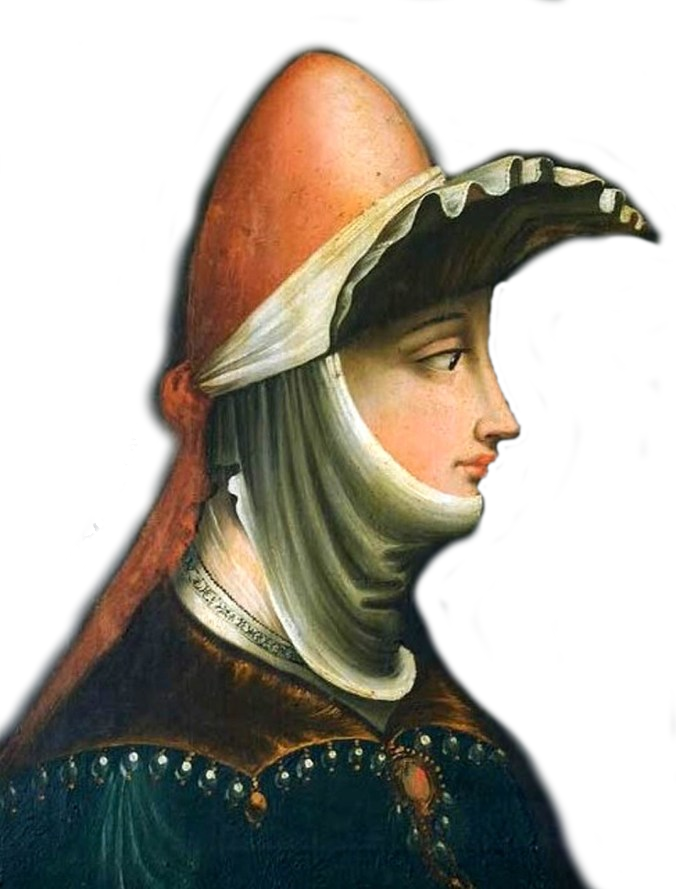
\includegraphics[width=7.5cm]{img/matilde.png}
    \caption{\textsf{Parmigianino, Ritratto di Matilde di Canossa, XVI secolo, Museo Diocesano, Mantova}}
    \label{fig:matilde}
\end{figure}

\subsection{Eventi storici}
Il contesto storico può essere raccontato ai PG quando il DM riterrà sia il momento migliore. Ad esclusione della missione dei PG e del personaggio di Tobaldo Malatesta, i fatti riportati sopra sono eventi storici realmente accaduti. Di seguito viene riportato cosa successe realmente a Matilde dopo il ritorno al Castello di Canossa. Questi eventi non fanno parte dell'avventura, ma posso essere utili al DM per comprendere meglio l'idea che sta alla base della oneshot.

Tra il 1073 e il 1074 il marito Goffredo il Gobbo scese nella penisola italiana per riconquistare Matilde offrendole possedimenti e armate, ma la risposta della Grancontessa fu estremamente ferma e rigida. Sul suo atteggiamento si è costruito il mito di una donna priva di debolezze.

Goffredo il Gobbo nel 1076 cadde vittima di un'imboscata nelle sue terre nei pressi di Anversa. Durante la notte, spinto da bisogni corporali, si recò al gabinetto e un sicario che stava in agguato gli conficcò una spada tra le natiche lasciandogli l'arma piantata nella ferita. Sembrava dovesse sopravvivere, ma una settimana dopo, il 27 febbraio 1076, morì, lasciando Matilde vedova. Molti commentatori dell'epoca l'accusarono di essersi macchiata personalmente del crimine; comunque come colpevole viene indicato più verosimilmente il conte fiammingo Roberto I delle Fiandre. In ogni caso Matilde non versò al clero neppure un obolo per l'anima del marito ucciso, né fece recitare una messa o gli dedicò un convento, com'era invece d'uso fare tra i nobili. 

\begin{figure}
\centering
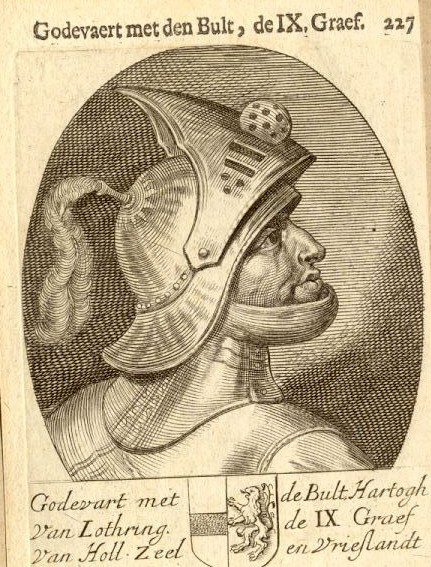
\includegraphics[width=7.5cm]{img/goffredo-il-gobbo.png}
    \caption{\textsf{Goffredo IV di Lorena detto ''il Gobbo''}}
    \label{fig:goffredo}
\end{figure}

\section{La missione}
È il 26 dicembre del 1073, i PG sono stati incaricati da Tobaldo Malatesta, servitore di alto rango della casata dei Canossa, di scortare un carro di provviste fino al Castello di Canossa. Il carro contiene prosciutti, salami, culatelli e forme di formaggio stagionato destinati alla festa di fine anno che si svolgerà al castello. Oltre ai viveri Tobaldo consegna una pergamena sigillata al paladino del gruppo che ha un background da messaggero, che dovrà consegnare personalmente a Matilde e dovrà proteggerne la segretezza anche a costo della propria vita.

Un personaggio del gruppo invece avrà una missione segreta diversa. Questo PG è un sicario incaricato da Roberto I delle Fiandre il quale lo ha pagato in anticipo 200 monete d'oro per uccidere Goffredo il Gobbo, \textbf{nobile} con 32 PF (Manuale dei Mostri p.349 \cite{dnd:mostri}) che alloggia al Castello di Canossa. Il sicario è riuscito ad infiltrarsi nel gruppo di corrieri per il trasporto di viveri al Castello, tuttavia la sua missione è una missione omicida.


\section{PG in breve}

\paragraph{Isabella Grattaciotoli} Ha 28 anni, è una \textit{halfling ladra}. Non particolarmente forte ma molto abile a nascondersi e particolarmente agile. Orfana di entrambi i genitori ha accettato di partecipare a questa missione perché la ricompensa le parmetterà di provvedere al sostegno dei suoi fratelli per tutto l'inverno. Difetti: quando vede dei dolci perde letteralmente la testa.

\paragraph{Dante Passafiume} È un \textit{paladino umano} di 50 anni, un veterano che fa parte della rete di messaggeri. Una persona coraggiosa e dall'alta integrità morale. Dante, se prende un impegno, lo porta a termine. Difetti: si irrita quando viene contraddetto.

\paragraph{Caterina Portinari} Caterina ha 25 anni ed è la più giovane del gruppo. Viene da una famiglia benestante. I genitori avrebbero voluto educarla per diventare una signora, una damigella, ma lei è una donna di azione. Fuggita dalla famiglia, ha studiato per un paio d'anni armi e tattiche di cobattimento e ora è un'abile \textit{guerriera umana}. Difetti: quando si tratta di finire un nemico esita.

\paragraph{Virgilio Monforte} È uno \textit{stregone mezz'elfo} anziano di 132 anni. Ha sempre messo i suoi innati poteri al servizio dei nobili del territorio. Difetti: a volte perde la testa e usa incantesimi totalmente inutili.

\paragraph{Clara Spina} Clara ha 35 anni, è una umana chierica, appartiene al dominio della vita, la sua missione è aiutare gli altri. Difetti: è una irrefrenabile pettegola.

\paragraph{Olin (nome di copertura Herbert Mann)} È un \textit{umano ladro} di 43 anni ma ufficialmente bardo con uno strumento rotto. È un sicario infiltrato nel gruppo per uccidere Goffredo il Gobbo. Difetti: è irritato dai nobili altezzosi, anche se riesce a trattenersi, a volte la sua irritazione traspare.




\subsection{NPC in breve}

\paragraph{Tobaldo Malatesta} Servitore di alto rango di Matilde. Gentile, una persona abituata a comandare, conosce Dante Passafiume.

\paragraph{Filippo Pocaterra} Oste della Locanda del cane zoppo di San Polo. Gentile ma non è la persona più pulita del regno. L'igiene non è la sua specialità.

\paragraph{Desiderio Forgiaferro} Mago anziano estremamente gentile e servizievole, brama di tradire Matilde e vorrebbe ingraziarsi i suoi nemici sperando di ricevere maggiore fortuna economica.

\paragraph{Matilde di Canossa} La Grancontessa ha 25 anni, ha la fama di essere una donna dura tutta di un pezzo...

\paragraph{Goffredo il Gobbo} Ha una vistosa gobba ma di fatto è una persona massiccia che sa difendersi. Non è la persona più simpatica del mondo. Era venuto in Italia per riconquistare Matilde promettendole terre ma Matilde lo ha rifiutato. Considera Matilde una lurida sgualdrina.


\chapter{L'arrivo al villaggio}
\DndDropCapLine{I}{ PG stanno trasportando} un carico di viveri e una pergamena con un messaggio segreto da consegnare di persona a Matilde. La missiva è in custodia al paladino che deve difenderla a costo della vita.

Leggi quanto segue per introdurli alla storia.

\begin{DndReadAloud}
Siamo nell'anno del Signore 1073. Oggi è il 26 dicembre. L'inverno è iniziato da poco ma sta già colpendo duramente. La neve cade spinta dal vento in tutte le direzioni come in una vera bufera. Sono le 5 del pomeriggio il sole che non si è visto per tutto il giorno è da poco sceso all'orizzonte e il grigio del cielo si sta trasformando rapidamente in nero. Una giornata ideale per mettersi seduti con i piedi al calduccio davanti al camino e mangiarsi una ciotola di stufato di maiale sotto una calda coperta. Purtroppo la sorte aveva altri piani per voi. Vi trovate nella tormenta a scortare un carro nella nebbia, nel turbinare della neve e con il buio che avanza con rapidità.

Clara conduce il carretto trainato da un mulo stanco che arranca nella neve alta una ventina di centimetri. Al fianco di Clara è seduto Virgilio che guarda avanti, ha lo sguardo perso e la sua mente sta viaggiando lontano. Forse in un luogo caldo? Davanti al carro Dante, il vostro paladino conduce il gruppo ed è scortato da Herbert che lo segue a pochi metri di distanza. 
\end{DndReadAloud}

Descrivi la disposizione dei PG rispetto al carro.

\begin{DndReadAloud}
Il carro procede a rilento, le ruote faticano ad affondare nella neve. Davanti a voi scorgete un ponte in legno dall'aspetto robusto oltre il ponte fanno capolino le luci di un piccolo villaggio: \textit{Plebs de Caviliano}. La vostra comitiva avanza. Percepite di essere sul ponte poiché il rumore sordo delle ruote del carro e del vostro mulo rimbomba leggermente sulle robuste assi di legno. Alcuni di voi hanno già attraversato questo fiume e lo conoscono molto bene. Un fiume che oggi sembra scomparso perché scorre sotto una coltre di ghiaccio ricoperto da uno strato di neve. Si tratta del Fiume Enza e, come vi dicevo, il villaggio di fronte a voi è  \textit{Plebs de Caviliano} che ai giorni nostri è noto come San Polo.
\end{DndReadAloud}

A questo punto probabilmente i PG si staranno chiedendo cosa trasportano.

\begin{DndReadAloud}
Vi starete chiedendo cosa trasporta il vostro carro. Un carro abbastanza grande coperto da un pesante tendone per proteggere la merce trasportata. Per capire cosa trasporta il carro dobbiamo tornare indietro di qualche ora, nella città di Parma, dove avete incontrato Tobaldo Malatesta, servitore di alto rango della casata dei Canossa. Tobaldo una persona gentile ma evidentemente abituata al comando, vi ha incaricato di trasportare un carico di viveri al castello di Canossa al quale dovete arrivare entro il 29 dicembre. Il carro contiene cosce di maiale stagionate, salami di maiale e culatelli prodotti dai lardaroli di Parma; svariate caciotte e una grossa forma di formaggio stagionato che il monastero benedettino di San Giovanni Evangelista ha provato a produrre lo scorso anno e sembra essere molto buono. Questo goloso carico servirà per la festa di fine anno che si volgerà al castello.

Tobaldo ha preso in disparte il vostro paladino per consegnargli una pergamena che Dante dovrà consegnare personalmente a Matilde. Tobaldo, posando una mano sulla spalla di Dante ha pronunciato alcune parole che tutto il vostro gruppo ha potuto sentire <<Mio caro Dante, appartieni da alcuni anni alla rete di messaggeri e la tua fama in battaglia ti precede ovunque vai. Custodisci la segretezza di questa missiva destinata alla Grancontessa a costo della tua stessa vita e comanda il tuo gruppo per raggiungere il tuo obiettivo>>
\end{DndReadAloud}

Nel pomeriggio, dopo aver ricevuto l'incarico da Tobaldo, il gruppo è partito nella tormenta per raggiungere l'abitato di San Polo dove fare tappa.


\DndFeatHeader{Il carro al sicuro}
All'arrivo al villaggio di San Polo i PG saranno costretti ad alloggiare alla locanda per trascorrere la notte ed eventualmente attendere il passaggio della tormenta. Nella locanda troveranno alcuni NPC che racconteranno quanto il DM vorrà della storia riportata all'inizio del presente testo.

\begin{DndReadAloud}
Quando entrate nella locanda affollata, il brusio di abbassa istantaneamente e alcuni ospiti si girano per osservarvi incuriositi. La maggior parte di loro sono contadini. All'ingresso un misto di odore stufato, legna bruciata, letame e sudore arriva alle vostre narici. L'oste vi fa un caloroso sorriso dietro ai suoi baffoni.
\end{DndReadAloud}

L'oste, Filippo Pocaterra (\textbf{popolano}), darà il massimo delle rassicurazioni ai PG garantendo che nessuno potrà toccare i viveri presenti sul carro in quanto saranno posizionati in una stalla che verrà chiusa con un pesante lucchetto.

L'oste offrirà loro una camera agiata è una sostanziosa cena al costo di 8 ma. Per la cena potranno scegliere fra stufato di maiale o pollo alla cacciatore e una caraffa di vino rosso.

I PG che mangeranno lo stufato di maiale, prima di coricarsi, dovranno fare un TS su costituzione con CD 11, se non lo superano, si ammalano di Epidemia fognaria (Manuale del DM, p.257 \cite{dnd:dm})). I PG ammalati il giorno dopo saranno Indeboliti (Manuale del Gocatore p.291 \cite{dnd:giocatore}) al livello 1 ma potranno rifare un TS su costituzione per vedere se l'indebolimento peggiora o miglioa. Al termine di ogni riposo lungo successivo, potranno rifare il TS per vedere se la malattia si aggrava o no, non potranno recuperare PF ma potranno tirare un dado vita ogni riposo breve di almeno 1 ora aggiungendo metà punteggio.

\begin{DndTable}[color=PhbLightCyan,header=Indebolimento]{cX}
  \textbf{Liv.} & \textbf{Effetto} \\
  1 & Svantaggio alle prove di caratteristica \\
  2 & Velocità dimezzata \\
  3 & Svantaggio ai tiri per colpire e ai TS \\
  4 & Massimo dei punti ferita dimezzato \\
  6 & Velocità ridotta a 0 \\
  7 & Morte \\
\end{DndTable}


\chapter{Verso Canossa}
\DndDropCapLine{L}{a tormenta è passata.} I PG si risvegliano in una limpida giornata ivernale. L'aria è gelida e luminosa e il paesaggio è completamente ammantato di bianco. Guardando a Nord sono in grado di vedere la foresta che si estende nella pianura e in fondo sono debolmente visibili le Alpi anche loro ammantate di neve.

Quando i PG partiranno alla volta del Castello di Canossa, potranno scegliere due strade: portarsi verso Quattrocastella e salire a Canossa oppure proseguire lungo la valle dell'Enza e poi salira a Est verso Canossa.

\section{Banditi}
I PG troveranno sul terreno un finto cadavere. Quando scenderanno dal carro saranno circondati da 2 \textbf{banditi} più il \textbf{capo dei banditi}.

\section{Il mago traditore}
Mentre i PG viaggiano verso il castello di Canossa, scorgono davanti a loro delle impronte nella neve sono impronte di umano. Se indagano possono scoprire che l'umano ha un bastone e trascina un piede.

L'umano è uno dei consiglieri di Matilde diretto a Canossa. Si tratta di un \textbf{mago} (Manuale dei Mostri p.348 \cite{dnd:mostri}) che ha tutta l'intenzione di tradire Matilde. 

\begin{DndSidebar}{Interpretare il mago}
Il mago è vecchio e affaticato. Deve far credere ai PG che se prosegue nella neve rischia di morire. Racconterà che è stato rapinato dai banditi che gli hanno rubato il mulo e tutti i suoi averi. È diretto al castello perché è stato invitato da Matilde come consigliere per la festa di fine anno.
\end{DndSidebar}

Il mago è stato informato che un certo numero di avventurieri è stato incaricato di portare un carico di viveri a Canossa. Uno di questi avventurieri ha un messaggio segreto, non sa chi sia il messaggero.

Per prima cosa proverà a capire se sono il gruppo di avventurieri che trasporta il cibo a Canossa.

Se capirà che sono loro proverà a lanciare l'incantesimo \textit{suggestione} all'halfling del gruppo parlandole in halfling.


\begin{DndReadAloud}
Mia cara, era da molto che non vedevo un halfling da queste parti. Da dove provieni?
Saresti così gentile da fare una cosa per me? Mia cara, mi risulta che state trasportando un messaggio per Matilde. Quando ritieni più opportuno dovresti leggere il messaggio e riferirmi il contenuto. TS 14
\end{DndReadAloud}


\section{Udienza con Matilde}

\chapter{Appendice}
\section{Il testo della pergamena}

\subparagraph{Subparagraph}
The subparagraph format with the paragraph indent is likely going to be more familiar to the reader.

\section{Special Sections}
The module also includes functions to aid in the proper typesetting of multi-line section headers: |\DndFeatHeader| for feats, |\DndItemHeader| magic items and traps, and |\DndSpellHeader| for spells.

\DndFeatHeader{Typesetting Savant}[Prerequisite: \LaTeX{} distribution]
You have acquired a package which aids in typesetting source material for one of your favorite games. You have advantage on Intelligence checks to typeset new content. On a failed check, you can ask questions online at the package's website.

\DndItemHeader{Foo's Quill}{Wondrous item, rare}
This quill has 3 charges. While holding it, you can use an action to expend 1 of its charges. The quill leaps from your hand and writes a contract applicable to your situation.

The quill regains 1d3 expended charges daily at dawn.

\DndSpellHeader%
  {Beautiful Typesetting}
  {4th-level illusion}
  {1 action}
  {5 feet}
  {S, M (ink and parchment, which the spell consumes)}
  {Until dispelled}
You are able to transform a written message of any length into a beautiful scroll. All creatures within range that can see the scroll must make a wisdom saving throw or be charmed by you until the spell ends.

While the creature is charmed by you, they cannot take their eyes off the scroll and cannot willingly move away from the scroll. Also, the targets can make a wisdom saving throw at the end of each of their turns. On a success, they are no longer charmed.

%\begin{figure*}
%    \centering
%    \includegraphics[width=\textwidth]{test.png}
%    \caption{\textsf{The structure of our tic-tac-toe implementation.}}
%    \label{fig:ds}
%\end{figure*}

\lipsum[3-10]

\section{Map Regions}
The map region functions |\DndArea| and |\DndSubArea| provide automatic numbering of areas.

\DndArea{Village of Hommlet}
This is the village of hommlet.

\DndSubArea{Inn of the Welcome Wench}
Inside the village is the inn of the Welcome Wench.

\DndSubArea{Blacksmith's Forge}
There's a blacksmith in town, too.

\DndArea{Foo's Castle}
This is foo's home, a hovel of mud and sticks.

\DndSubArea{Moat}
This ditch has a board spanning it.

\DndSubArea{Entrance}
A five-foot hole reveals the dirt floor illuminated by a hole in the roof.

\chapter{Text Boxes}

The module has three environments for setting text apart so that it is drawn to the reader's attention. |DndReadAloud| is used for text that a game master would read aloud.

\begin{DndReadAloud}
  As you approach this module you get a sense that the blood and tears of many generations went into its making. A warm feeling welcomes you as you type your first words.
\end{DndReadAloud}

\section{As an Aside}
The other two environments are the |DndComment| and the |DndSidebar|. The |DndComment| is breakable and can safely be used inline in the text.

\begin{DndComment}{This Is a Comment Box!}
  A |DndComment| is a box for minimal highlighting of text. It lacks the ornamentation of |DndSidebar|, but it can handle being broken over a column.
\end{DndComment}

The |DndSidebar| is not breakable and is best used floated toward a page corner as it is below.

\begin{DndSidebar}[float=!b]{Behold the DndSidebar!}
  The |DndSidebar| is used as a sidebar. It does not break over columns and is best used with a figure environment to float it to one corner of the page where the surrounding text can then flow around it.
\end{DndSidebar}

\section{Tables}
The |DndTable| colors the even rows and is set to the width of a line by default.

\begin{DndTable}[header=Nice Table]{XX}
    \textbf{Table head}  & \textbf{Table head} \\
    Some value  & Some value \\
    Some value  & Some value \\
    Some value  & Some value
\end{DndTable}

\chapter{Monsters and NPCs}

% Monster stat block
\begin{DndMonster}[float*=b,width=\textwidth + 8pt]{Monster Foo}
  \begin{multicols}{2}
    \DndMonsterType{Medium aberration (metasyntactic variable), neutral evil}

    % If you want to use commas in the key values, enclose the values in braces.
    \DndMonsterBasics[
        armor-class = {9 (12 with \emph{mage armor})},
        hit-points  = {\DndDice{3d8 + 3}},
        speed       = {30 ft., fly 30 ft.},
      ]

    \DndMonsterAbilityScores[
        str = 12,
        dex = 8,
        con = 13,
        int = 10,
        wis = 14,
        cha = 15,
      ]

    \DndMonsterDetails[
        %saving-throws = {Str +0, Dex +0, Con +0, Int +0, Wis +0, Cha +0},
        %skills = {Acrobatics +0, Animal Handling +0, Arcana +0, Athletics +0, Deception +0, History +0, Insight +0, Intimidation +0, Investigation +0, Medicine +0, Nature +0, Perception +0, Performance +0, Persuasion +0, Religion +0, Sleight of Hand +0, Stealth +0, Survival +0},
        %damage-vulnerabilities = {cold},
        %damage-resistances = {bludgeoning, piercing, and slashing from nonmagical attacks},
        %damage-immunities = {poison},
        %condition-immunities = {poisoned},
        senses = {darkvision 60 ft., passive Perception 10},
        languages = {Common, Goblin, Undercommon},
        challenge = 1,
      ]
    % Traits
    \DndMonsterAction{Innate Spellcasting}
    Foo's spellcasting ability is Charisma (spell save DC 12, +4 to hit with spell attacks). It can innately cast the following spells, requiring no material components:
    \begin{DndMonsterSpells}
      \DndInnateSpellLevel{misty step}
      \DndInnateSpellLevel[3]{fog cloud, rope trick}
      \DndInnateSpellLevel[1]{identify}
    \end{DndMonsterSpells}

    \DndMonsterAction{Spellcasting}
    Foo is a 2nd-level spellcaster. Its spellcasting ability is Charisma (spell save DC 12, +4 to hit with spell attacks). It has the following sorcerer spells prepared:
    \begin{DndMonsterSpells}
      \DndMonsterSpellLevel{blade ward, fire bolt, light, shocking grasp}
      \DndMonsterSpellLevel[1][3]{burning hands, mage armor, shield}
    \end{DndMonsterSpells}

    \DndMonsterSection{Actions}
    \DndMonsterAction{Multiattack}
    The foo makes two melee attacks.

    %Default values are shown commented out
    \DndMonsterAttack[
      name=Dagger,
      %distance=both, % valid options are in the set {both,melee,ranged},
      %type=weapon, %valid options are in the set {weapon,spell}
      mod=+3,
      %reach=5,
      %range=20/60,
      %targets=one target,
      dmg=\DndDice{1d4+1},
      dmg-type=piercing,
      %plus-dmg=,
      %plus-dmg-type=,
      %or-dmg=,
      %or-dmg-when=,
      %extra=,
    ]

    %\DndMonsterMelee calls \DndMonsterAttack with the melee option
    \DndMonsterMelee[
      name=Flame Tongue Longsword,
      mod=+3,
      %reach=5,
      %targets=one target,
      dmg=\DndDice{1d8+1},
      dmg-type=slashing,
      plus-dmg=\DndDice{2d6},
      plus-dmg-type=fire,
      or-dmg=\DndDice{1d10+1},
      or-dmg-when=if used with two hands,
      %extra=,
    ]

    %\DndMonsterRanged calls \DndMonsterAttack with the ranged option
    \DndMonsterRanged[
      name=Assassin's Light Crossbow,
      mod=+1,
      range=80/320,
      dmg=\DndDice{1d8},
      dmg-type=piercing,
      %plus-dmg=,
      %plus-dmg-type=,
      %or-dmg=,
      %or-dmg-when=,
      extra={, and the target must make a DC 15 Constitution saving throw, taking 24 (7d6) poison damage on a failed save, or half as much damage on a successful one}
    ]

    % Legendary Actions
    \DndMonsterSection{Legendary Actions}
    The foo can take 3 legendary actions, choosing from the options below. Only one legendary action option can be used at a time and only at the end of another creature's turn. The foo regains spent legendary actions at the start of its turn.

    \begin{DndMonsterLegendaryActions}
      \DndMonsterLegendaryAction{Move}{The foo moves up to its speed.}
      \DndMonsterLegendaryAction{Dagger Attack}{The foo makes a dagger attack.}
      \DndMonsterLegendaryAction{Create Contract (Costs 3 Actions)}{The foo presents a contract in a language it knows and waves it in the face of a creature within 10 feet. The creature must make a DC 10 Intelligence saving throw. On a failure, the creature is incapacitated until the start of the foo's next turn. A creature who cannot read the language in which the contract is written has advantage on this saving throw.}
    \end{DndMonsterLegendaryActions}
  \end{multicols}
\end{DndMonster}

The |DndMonster| environment is used to typeset monster and NPC stat blocks. The module supplies many functions to easily typeset the contents of the stat block

\chapter{Colors}

\begin{table*}[b]%
  \caption{}\label{tab:colors}

  \begin{DndTable}[width=\linewidth,header=Colors Supported by This Package]{lX}
    \textbf{Color}                  & \textbf{Description} \\
    |PhbLightGreen|                 & Light green used in PHB Part 1 (Default) \\
    |PhbLightCyan|                  & Light cyan used in PHB Part 2 \\
    |PhbMauve|                      & Pale purple used in PHB Part 3 \\
    |PhbTan|                        & Light brown used in PHB appendix \\
    |DmgLavender|                   & Pale purple used in DMG Part 1 \\
    |DmgCoral|                      & Orange-pink used in DMG Part 2 \\
    |DmgSlateGray| (|DmgSlateGrey|) & Blue-gray used in PHB Part 3 \\
    |DmgLilac|                      & Purple-gray used in DMG appendix \\
  \end{DndTable}
\end{table*}

This package provides several global color variables to style |DndComment|, |DndReadAloud|, |DndSidebar|, and |DndTable| environments.

\begin{DndTable}[header=Box Colors]{lX}
  \textbf{Color}   & \textbf{Description} \\
  |commentcolor|   & |DndComment| background \\
  |readaloudcolor| & |DndReadAloud| background \\
  |sidebarcolor|   & |DndSidebar| background \\
  |tablecolor|     & background of even |DndTable| rows \\
\end{DndTable}

They also accept an optional color argument to set the color for a single instance. See Table~\ref{tab:colors} for a list of core book accent colors.

\begin{lstlisting}
\begin{DndTable}[color=PhbLightCyan]{cX}
  \textbf{d8} & \textbf{Item} \\
  1 & Small wooden button \\
  2 & Red feather \\
  3 & Human tooth \\
  4 & Vial of green liquid \\
  6 & Tasty biscuit \\
  7 & Broken axe handle \\
  8 & Tarnished silver locket \\
\end{DndTable}
\end{lstlisting}

\begin{DndTable}[color=PhbLightCyan]{cX}
  \textbf{d8} & \textbf{Item} \\
  1 & Small wooden button \\
  2 & Red feather \\
  3 & Human tooth \\
  4 & Vial of green liquid \\
  6 & Tasty biscuit \\
  7 & Broken axe handle \\
  8 & Tarnished silver locket \\
\end{DndTable}

\section{Themed Colors}
Use |\DndSetThemeColor[<color>]| to set |commentcolor|, |readaloudcolor|, |sidebarcolor|, and |tablecolor| to a specific color. Calling |\DndSetThemeColor| without an argument sets those colors to the current |themecolor|. In the following example the group limits the change to just a few boxes; after the group finishes, the colors are reverted to what they were before the group started.

\begin{lstlisting}
\begingroup
\DndSetThemeColor[PhbMauve]

\begin{DndComment}{This Comment Is in Mauve}
  This comment is in the the new color.
\end{DndComment}

\begin{DndSidebar}{This Sidebar Is Also Mauve}
  The sidebar is also using the new theme color.
\end{DndSidebar}
\endgroup
\end{lstlisting}

\begingroup
\DndSetThemeColor[PhbMauve]

\begin{DndComment}{This Comment Is in Mauve}
  This comment is in the the new color.
\end{DndComment}

\begin{DndSidebar}{This Sidebar Is Also Mauve}
  The sidebar is also using the new theme color.
\end{DndSidebar}
\endgroup


\bibliography{bibliografia}{}
\bibliographystyle{plain}

\end{document}

